%Suitability of Exciters for Perceptual Control
%	Parameterise feature changes in terms of harmonic excitation.
%	Most suitable methods for given feature manipulations.
%	Easiest features to control in isolation.

\chapter{Controlling Audio Features} % control of low level features using exciters
\label{chap:FeatureControl}

\section{Introduction}
\label{sec:FeatureControl-Introduction}
	Previous studies, discussed in Section~\ref{sec:Timbre-Control}, have attempted to control perceptual features,
	such as warmth and brightness, by controlling specific audio features. The characteristics of the harmonic
	excitation systems discussed in Chapter~\ref{chap:ExcitationEvaluation} can be utilised to provide similar control
	over audio features. Ideally, control over a feature should be linear (the relationship between the effect's
	parameter setting the feature value being linear) and independent (the effect only controls one audio feature, the
	rest remaining constant). This would allow for the most flexibility in applying timbral transforms, every separate
	feature can be set individually and predictably. In reality this is not achievable: providing linear control
	requires in depth analysis of the input signal which cannot be applied in real time. In addition, independent
	control of features is not always possible as several features are closely related, such as spectral flatness and
	spectral irregularity. In light of this, the techniques developed in this chapter will focus on providing monotonic
	control over an audio feature: a given direction in change of parameter setting will always produce the same
	direction of change of the audio feature.
	
	This chapter will provide methods by which several audio features can be controlled through harmonic excitation and
	which excitation algorithms are the most suitable for given feature changes. Firstly, in
	Section~\ref{sec:FeatureControl-Systems}, various challenges which arise when building harmonic excitation systems
	are discussed and methods to counteract them are suggested. A number of different systems are proposed which
	provide control over the nature of the new frequency components introduced to the signal. In
	Section~\ref{sec:FeatureControl-Parameterisation} methods by which these systems can be configured to provide
	monotonic control over specific audio features are proposed and tested.

\section{Harmonic Excitation Systems}
\label{sec:FeatureControl-Systems}
	In Section~\ref{sec:Excitation-Methods} several different methods of introducing new frequency content to a signal
	were introduced. In Section~\ref{sec:ExcitationEvaluation-Comparison} these methods were discussed further and the
	degree to which their effect can be controlled evaluated. From that analysis it is known that better control over
	the output is gained through meeting certain input requirements, for instance the SSBA and IAP techniques will
	produce sinusoidal outputs for sinusoidal inputs. It is also noted that further filtering may be needed after the
	use of a harmonic excitation algorithms in order to shape the spectrum as desired, such as after a peak clipper has
	been applied. Harmonic excitation systems can be constructed which apply these pre and post-processing before and
	after a giver harmonic excitation algorithm. This section discusses the design of these systems, aiming to give
	users precise control over the new spectral content added to a wide range of input signals.

	\subsection{$f_{0}$ Tracking}
	\label{sec:FeatureControl-Systems-Fundamental}
		As discussed in Section~\ref{sec:ExcitationEvaluation-Comparison}, the behaviour of several of the harmonic
		excitation systems is more predictable for sinusoidal inputs. This is due to the elimination of
		intermodulation distortion components by having an input signal consisting of only a single frequency. This
		more predictable behaviour simplifies the problem of using harmonic excitation algorithms in providing
		monotonic control of audio features, allowing similar transforms to be applied to a wide range of input
		signals. To take advantage of these improvement in predictability the input signal to a harmonic exciter
		must be pre-processed such that it is represented by a single sinusoid. For monophonic tonal sources this
		can be achieved by representing this signal as a sinusoid at the input's $f_{0}$. This remainder of this
		thesis then focusses of controlling timbre in this class of audio signal. Other classes of signal
		(polyphonic, noisy etc.) are left for consideration in future work.
		
		A monophonic tonal signal can be represented as a sinusoid by applying a band pass filter centered around
		its $f_{0}$. This produces a narrowband signal with the majority of its energy concentrated at the $f_{0}$.
		In the following discussion this filtered signal will be referred to as the `isolated $f_{0}$'. Applying a
		harmonic excitation algorithm to the isolated $f_{0}$ will produce a signal with a lower level of
		intermodulation components than processing the original input signal. The `excited' isolated $f_{0}$ signal
		can then be summed with the original signal to produce the output. A diagram of this system is shown in
		Figure~\ref{fig:F0Tracking}.

		\begin{figure}[h!]
			\centering
			\begin{tikzpicture}
				\node (In) at (0, 1) {$x[n]$};
				\coordinate (InMid) at (1, 1);
				\draw (In) -- (InMid);

				\coordinate (Through) at (1, 0);
				\draw (InMid) -- (Through);
				\coordinate (ThroughOut) at (9, 0);
				\draw (Through) -- (ThroughOut);

				\coordinate (Side) at (1, 2);
				\draw (InMid) -- (Side);

				\node (F0) [draw] at (2.5, 2) {$f_{0}$ Tracker};
				\node (Filter) [draw] at (2.5, 1) {BPF};
				\draw (InMid) -- (Filter);
				\draw (F0) -- (Filter);

				\node (Exciter) [draw] at (5, 1) {Harmonic Exciter};
				\draw (Filter) -- (Exciter);
				\draw (Side) -- (F0);

				\node (Add) [operator] at (9, 1) {+};
				\draw (ThroughOut) -- (Add);

				\node (Gain) [gain] at (7.5, 1) {Gain};
				\draw (Exciter) -- (Gain);
				\draw (Gain) -- (Add);

				\node (Out) at (10.25, 1) {$y[n]$};
				\draw (Add) -- (Out);
			\end{tikzpicture}
			\caption{$f_{0}$ frequency tracking in a harmonic excitation system.}
			\label{fig:F0Tracking}
		\end{figure}

		For this system to operate in real time the $f_{0}$ of the signal must be calculated in real time. This is
		achieved using the $f_{0}$ tracker shown in the diagram. $f_{0}$ tracking is a widely researched field and
		several algorithms have been presented in the literature, several of which are reviewed by
		\citet{cuadra2001efficient} and \citet{gerhard2003pitch}.  $f_{0}$ tracking can be done in both the time
		and frequency domains. The simplest method being to count the number of instances of a particular event in
		a given time period. This event could be a zero crossing, a peak or any other easily identifiable feature
		of the signal. As signals get more complex, this method becomes more difficult to apply as higher frequency
		content will produce more instances of the event being counted. More advanced time domain methods include
		the Average Magnitude Difference Function (AMDF) and autocorrelation methods. Many modern $f_{0}$ tracking
		systems are based on these, such as the YIN method proposed by \citet{decheveigne2002yin} and the VT-AMDF
		algorithm proposed by \citet{prukkanon2009vt-amdf}.  These methods require frame based processing which
		reduces the time resolution of the system. If analysing real time audio the current estimate of the $f_{0}$
		will lag behind the audio signal. \citet{larsen2004audio} describe a time domain frequency tracker which
		uses a simple recursive formula. While this is not as precise as the more advanced techniques it takes
		considerably less time to compute. Frequency domain methods require the DFT of the signal to be calculated
		introducing considerable complexity. Widely used frequency domain techniques include the Harmonic Product
		Spectrum (HPS) and maximum likelihood estimate methods \citep{noll1969pitch}. State of the art techniques
		employ statistical / machine learning techniques to improve the performance of $f_{0}$ trackers for input
		signals with high levels of noise. These techniques include a probabilistic framework \citep{chu2012safe},
		artificial neural networks \citep{han2014neural} and hidden Markov models \citep{wang2016f0}. Other recent
		work has developed methods of tracking multiple pitches in polyphonic signals \citep{christensen2008multi}.
		Due to this work's focus on monophonic signals, these are beyond the scope of this discussion.

		For real time harmonic excitation, the accuracy of the $f_{0}$ tracking algorithm is not as important as it
		is in other fields such as automatic music transcription. The aim of the system in
		Figure~\ref{fig:F0Tracking} is to reduce the level of higher harmonics compared to the $f_{0}$. Using a low
		pass filter with a cutoff frequency close to the $f_{0}$ will achieve this. The lag between the audio and
		the estimate of the $f_{0}$ is of greater concern. The system needs to respond quickly to changes in
		$f_{0}$ in order to better isolate it for processing.

		A problem is posed by signals with little energy at their $f_{0}$, such as those produced in the lower
		register of a Double Bass \citep{askenfelt2010double}. An $f_{0}$ tracking algorithm will still return the
		frequency of the $f_{0}$ despite its low magnitude. The isolated $f_{0}$ may then have too little amplitude
		to be of any use for harmonic excitation. A frequency domain approach to $f_{0}$ tracking may be more
		robust in this situation as it is easier to check whether there is sufficient energy at the detected
		$f_{0}$. If there is not, the first harmonic which has sufficient magnitude can be isolated and used as the
		input to the exciter. If this action is taken, only the spectral replication and spectral shifting methods
		will allow for the excitation of every harmonic. The SSBA and IAP methods only allow for integer
		multiplications of the input frequency.

		The system shown in Figure~\ref{fig:F0Tracking} can provide differing levels of flexibility depending on
		the harmonic exciter used. Using a static nonlinearity will generate a series of harmonics of the $f_{0}$.
		Using methods which provide more control over the order of distortion allows users to excite single
		harmonics in the output. This will be covered in the next section.

	\subsection{Individual Harmonic Generation}
	\label{sec:FeatureControl-Systems-Individuals}
		Control over which harmonics are excited in a signal can be achieved by generating individual harmonics.
		The principle behind this is to isolate the $f_{0}$ and then shift its frequency to that of the desired
		harmonic, as done in the system shown in Figure~\ref{fig:HarmonicGenerationSystem}.  The frequency shifter
		in this system can be implemented using the SSBA, IAP, Spectral Replication or Spectral Stretching methods.

		\begin{figure}[h!]
			\centering
			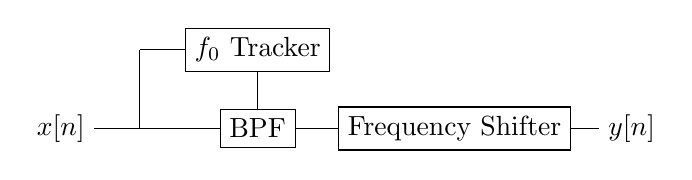
\begin{tikzpicture}
				\node (In) at (0, 1) {$x[n]$};
				\coordinate (InMid) at (1, 1);
				\draw (In) -- (InMid);

				\coordinate (Side) at (1, 2);
				\draw (InMid) -- (Side);

				\node (F0) [draw] at (2.5, 2) {$f_{0}$ Tracker};
				\node (Filter) [draw] at (2.5, 1) {BPF};
				\draw (InMid) -- (Filter);
				\draw (F0) -- (Filter);

				\node (Exciter) [draw] at (5, 1) {Frequency Shifter};
				\draw (Filter) -- (Exciter);
				\draw (Side) -- (F0);

				\node (Out) at (7.25, 1) {$y[n]$};
				\draw (Exciter) -- (Out);
			\end{tikzpicture}
			\caption{Generating individual harmonics for a signal.}
			\label{fig:HarmonicGenerationSystem}
		\end{figure}

		A complex spectrum can be created by generating several different order harmonics in this manner and
		summing them together. \citet{bregman1994auditory} suggests that when presented with an auditory scene the
		human hearing system separates out sources by grouping like harmonics together. Whether harmonics are
		deemed to be similar depends on their frequency and amplitude envelopes. When applying harmonic excitation
		it is necessary to ensure that the newly introduced harmonic content will be judged as similar to the
		existing content. If not, the excited harmonics may be perceived as a new sound source rather than
		contributing towards changing the timbre of a sound. Any system which generates new harmonic content and
		then sums it back into the original signal is at risk of this occurring. When generating multiple harmonics
		individually and summing them all together this risk is increased. Minimising the number of individual
		harmonics generated limits the problems arising from this as well as decreasing the computational load. The
		following section discusses how a system can be constructed which provides sufficient control over the
		shape of a spectrum while limiting the number of harmonics generated individually.
		
	\subsection{Spectral Shaping}
	\label{sec:FeatureControl-Systems-SpectralShaping}
		As seen in Section~\ref{sec:ExcitationEvaluation-Comparison-SpectralCharacteristics}, static nonlinearities
		provide an efficient way to generate large numbers of harmonics for sinusoidal inputs. The characteristic
		curve of the nonlinearity can be designed to produce a set of harmonics with the desired qualities, the
		parity of the characteristic curve can be used to control whether odd or even harmonics are generated and
		the `smoothness' of the curve can be adjusted to control the roll off of the harmonics' amplitudes. The
		shape of the generated spectrum can then be further shaped by filtering.

		A spectral shaping system can be constructed in which a static nonlinearity and filter are used to excite a
		large band of harmonics and finer control is provided using the individual harmonic generation method shown
		in Figure~\ref{fig:HarmonicGenerationSystem}. This allows the majority of the harmonics to be excited in an
		efficient manner, only using more complex processing where it is needed. \citet{howard2009acoustics} show
		that low order harmonics sit in separate critical bands, whereas high order harmonics are within one
		critical bandwidth of one another. This means that lower order harmonics are resolved separately by the
		human hearing system, while the high order harmonics are perceived as fused sounds. As the order of
		harmonics increases, their individual amplitudes have less effect on the perceived timbre of the sound. For
		this reason, a harmonic excitation system need only provide control over the individual amplitudes of low
		order harmonics. 

		Using Equation~\ref{eq:ERB}, the minimum order for which harmonics lie within one critical bandwidth of one
		another can be calculated. For a signal with a given $f_{0}$, this order, $n$, can be calculated using the
		inequality in Equation~\ref{eq:MinimumFusedHarmonic}.

%		\begin{gather}
%			f_{0} < 24.7 \left( 4.37n \frac{f_{0}}{1000} + 1 \right) \nonumber \\
%			n > 1000 \frac{f_{0} - 24.7}{24.7 \times 4.37f_{0}}
%			\label{eq:MinimumFusedHarmonic}
%		\end{gather}

		\begin{equation}
			n > 1000 \frac{f_{0} - 24.7}{24.7 \times 4.37f_{0}}
			\label{eq:MinimumFusedHarmonic}
		\end{equation}

		This value is dependent on the $f_{0}$ of the signal. As $f_{0}$ rises, the minimum value of $n$ grows
		asymptotically towards 9.26 as shown in Equation~\ref{eq:IndividualHarmonicLimit}.

		\begin{equation}
			\lim_{f_{0} \to \infty} 1000 \frac{f_{0} - 24.7}{24.7 \times 4.37f_{0}} \approx 9.26
			\label{eq:IndividualHarmonicLimit}
		\end{equation}

		For any value of $f_{0}$, a maximum of nine harmonics will lie at least one critical bandwidth away from
		all other harmonics. The individual amplitudes of the tenth, and higher order, harmonics have less effect
		on the timbre of a signal. This leads to the system shown in Figure~\ref{fig:SpectralShapingSystem}, an
		expansion of the system shown in Figure~\ref{fig:F0Tracking} providing finer control over the amplitudes of
		the first nine harmonics. The $f_{0}$ is isolated in the same manner but several exciters are used in
		parallel. Each of the first nine harmonics are generated individually from the isolated $f_{0}$. Higher
		order harmonics are generated using a static nonlinearity and high pass filter in combination. The filter's
		primary purpose is to remove any energy present in the first nine harmonics but can also be used to alter
		the distribution of energy in the higher order harmonics.

		\begin{figure}[h!]
			\centering
			\begin{tikzpicture}
				\node (In) at (-1, -1.75) {$x[n]$};
				\coordinate (InMid) at (0, -1.75);
				\draw (In) -- (InMid);

				\coordinate (Side) at (0, -0.75);
				\draw (InMid) -- (Side);

				\node (F0) [draw] at (2, -0.75) {$f_{0}$ Tracker};
				\node (F0Filter) [draw] at (2, -1.75) {BPF};
				\draw (InMid) -- (F0Filter);
				\draw (F0) -- (F0Filter);
				\draw (Side) -- (F0);

				\node (Add) [operator] at (10.5, -1.75) {+};

				\coordinate (ExciterIn) at (4, -1.75);
				\draw (F0Filter) -- (ExciterIn);

				% the fundamental
				\coordinate (F0In) at (4, 1);
				\node (F0Gain) [gain] at (9, 1) {};
				\draw (F0In) -- (F0Gain);
				\coordinate (F0Out) at (9.5, 1);
				\draw (F0Gain) -- (F0Out);
				\draw (F0Out) -- (Add);

				% second harmonic
				\coordinate (F1In) at (4, 0);
				\draw (F0In) -- (F1In);
				\node (F1) [draw] at (6.5, 0) {2\super{nd} Harmonic};
				\draw (F1In) -- (F1);

				\node (F1Gain) [gain] at (9, 0) {};
				\draw (F1) -- (F1Gain);
				\coordinate (F1Out) at (9.5, 0);
				\draw (F1Gain) -- (F1Out);
				\draw (F1Out) -- (Add);

				% third harmonic
				\coordinate (F2In) at (4, -1);
				\draw (F1In) -- (F2In);
				\node (F2) [draw] at (6.5, -1) {3\super{rd} Harmonic};
				\draw (F2In) -- (F2);

				\node (F2Gain) [gain] at (9, -1) {};
				\draw (F2) -- (F2Gain);
				\coordinate (F2Out) at (9.5, -1);
				\draw (F2Gain) -- (F2Out);
				\draw (F2Out) -- (Add);

				% ninth harmonic
				\coordinate (F8In) at (4, -2.5);
				\draw (F2In) -- (F8In);
				\node (F8) [draw] at (6.5, -2.5) {9\super{th} Harmonic};
				\draw (F8In) -- (F8);

				\node (F8Gain) [gain] at (9, -2.5) {};
				\draw (F8) -- (F8Gain);
				\coordinate (F8Out) at (9.5, -2.5);
				\draw (F8Gain) -- (F8Out);
				\draw (F8Out) -- (Add);

				\draw [dots] (F2) -- (F8);
				\draw [dots] (F2Gain) -- (F8Gain);

				% high order harmonics
				\coordinate (HighIn) at (4, -3.5);
				\draw (F8In) -- (HighIn);
				\node (High) [draw] at (5.7, -3.5) {Nonlinear Device};
				\draw (HighIn) -- (High);

				\node (HighFilter) [draw] at (8, -3.5) {Filter};
				\draw (High) -- (HighFilter);

				\node (HighGain) [gain] at (9, -3.5) {};
				\draw (HighFilter) -- (HighGain);
				\coordinate (HighOut) at (9.5, -3.5);
				\draw (HighGain) -- (HighOut);
				\draw (HighOut) -- (Add);

				% through
				\coordinate (Through) at (0, -4.5);
				\draw (InMid) -- (Through);
				\node (ThroughGain) [gain] at (9, -4.5) {};
				\draw (Through) -- (ThroughGain);
				\coordinate (ThroughOut) at (9.5, -4.5);
				\draw (ThroughGain) -- (ThroughOut);
				\draw (ThroughOut) -- (Add);

				\node (Out) at (11.75, -1.75) {$y[n]$};
				\draw (Add) -- (Out);
			\end{tikzpicture}
			\caption{An excitation system for controlling spectral structure.}
			\label{fig:SpectralShapingSystem}
		\end{figure}

	\subsection{Superposition}
	\label{sec:FeatureControl-Systems-Superposition}
		When processing musical signals, additional challenges are met when attempting to shape the spectrum
		through excitation. One such challenge concerns the superposition of the existing harmonics in a signal and
		those produced by the excitation. In certain situations these two signals may cause destructive
		interference. Although the exciter is set to produce energy at a given harmonic, when the signals are
		summed the energy at this harmonic decreases. To calculate the final amplitude of a harmonic, after the
		excited signals have been summed with the original signal, the phases and amplitudes of that harmonic in
		the original and excited signals must be known. This involves performing a full spectral analysis on the
		input signal. 

		When using a system like that shown in Figure~\ref{fig:SpectralShapingSystem}, the phases and amplitudes of
		the excited harmonics depend on the phase and amplitude of the isolated $f_{0}$. Using the SSBA and IAP
		techniques to generate the $n$\super{th} harmonic, the phase of the output is $n$ times that of the input
		after the Hilbert transform filter has been applied. The phases of the harmonics produced by a static
		nonlinearity can be determined by calculating the Fourier series of a sinusoid with the nonlinearity
		applied. Calculating this in real time dramatically increases the computational complexity of the system.
		This complexity can be avoided by avoiding superposition of harmonics. This simplest way to achieve this is
		by discarding the original signal and constructing the output from only the $f_{0}$ and generated
		harmonics.  This destroys most of the timbral characteristics of a signal, completely reconstructing its
		spectrum. For situations where a dramatic alteration of timbre is desired this can be a useful technique
		but for more subtle timbral manipulations it is beneficial to preserve more of the original spectral
		structure.

		A less intrusive method is to filter energy out of the input signal only at the frequencies which are to be
		excited. For the system in Figure~\ref{fig:SpectralShapingSystem} this can be implemented using a series of
		notch filters tuned to the frequencies of the first nine harmonics and a low pass filter to attenuate any
		frequency above the ninth harmonic. These filters can be applied to the unexcited signal depending on which
		harmonics are being generated by the exciters. A diagram of a system which includes these filters is shown
		in Figure~\ref{fig:SuperpositionSystem}.

		\begin{figure}[h!]
			\centering
			\begin{tikzpicture}
				\node (In) at (-1, -1.75) {$x[n]$};
				\coordinate (InMid) at (0, -1.75);
				\draw (In) -- (InMid);

				\coordinate (Side) at (0, -0.75);
				\draw (InMid) -- (Side);

				\node (F0) [draw] at (2, -0.75) {$f_{0}$ Tracker};
				\node (F0Filter) [draw] at (2, -1.75) {BPF};
				\draw (InMid) -- (F0Filter);
				\draw (F0) -- (F0Filter);
				\draw (Side) -- (F0);

				\node (Add) [operator] at (10.5, -1.75) {+};

				\coordinate (ExciterIn) at (4, -1.75);
				\draw (F0Filter) -- (ExciterIn);

				% the fundamental
				\coordinate (F0In) at (4, 1);
				\node (F0Gain) [gain] at (9, 1) {};
				\draw (F0In) -- (F0Gain);
				\coordinate (F0Out) at (9.5, 1);
				\draw (F0Gain) -- (F0Out);
				\draw (F0Out) -- (Add);

				% second harmonic
				\coordinate (F1In) at (4, 0);
				\draw (F0In) -- (F1In);
				\node (F1) [draw] at (6.5, 0) {2\super{nd} Harmonic};
				\draw (F1In) -- (F1);

				\node (F1Gain) [gain] at (9, 0) {};
				\draw (F1) -- (F1Gain);
				\coordinate (F1Out) at (9.5, 0);
				\draw (F1Gain) -- (F1Out);
				\draw (F1Out) -- (Add);

				% third harmonic
				\coordinate (F2In) at (4, -1);
				\draw (F1In) -- (F2In);
				\node (F2) [draw] at (6.5, -1) {3\super{rd} Harmonic};
				\draw (F2In) -- (F2);

				\node (F2Gain) [gain] at (9, -1) {};
				\draw (F2) -- (F2Gain);
				\coordinate (F2Out) at (9.5, -1);
				\draw (F2Gain) -- (F2Out);
				\draw (F2Out) -- (Add);

				% ninth harmonic
				\coordinate (F8In) at (4, -2.5);
				\draw (F2In) -- (F8In);
				\node (F8) [draw] at (6.5, -2.5) {9\super{th} Harmonic};
				\draw (F8In) -- (F8);

				\node (F8Gain) [gain] at (9, -2.5) {};
				\draw (F8) -- (F8Gain);
				\coordinate (F8Out) at (9.5, -2.5);
				\draw (F8Gain) -- (F8Out);
				\draw (F8Out) -- (Add);

				\draw [dots] (F2) -- (F8);
				\draw [dots] (F2Gain) -- (F8Gain);

				% high order harmonics
				\coordinate (HighIn) at (4, -3.5);
				\draw (F8In) -- (HighIn);
				\node (High) [draw] at (5.7, -3.5) {Nonlinear Device};
				\draw (HighIn) -- (High);

				\node (HighFilter) [draw] at (8, -3.5) {Filter};
				\draw (High) -- (HighFilter);

				\node (HighGain) [gain] at (9, -3.5) {};
				\draw (HighFilter) -- (HighGain);
				\coordinate (HighOut) at (9.5, -3.5);
				\draw (HighGain) -- (HighOut);
				\draw (HighOut) -- (Add);

				% through
				\coordinate (Through) at (0, -4.5);
				\draw (InMid) -- (Through);
				\node (ThroughFilter) [draw] at (8, -4.5) {Filter};
				\draw (Through) -- (ThroughFilter);
				\node (ThroughGain) [gain] at (9, -4.5) {};
				\draw (ThroughFilter) -- (ThroughGain);
				\coordinate (ThroughOut) at (9.5, -4.5);
				\draw (ThroughGain) -- (ThroughOut);
				\draw (ThroughOut) -- (Add);

				\node (Out) at (11.75, -1.75) {$y[n]$};
				\draw (Add) -- (Out);
			\end{tikzpicture}
			\caption{The system from Figure~\ref{fig:SpectralShapingSystem} extended to allow for filtering of
				 the original signal.}
			\label{fig:SuperpositionSystem}
		\end{figure}

		Removing harmonics from the original signal loses any phase information that was present for those
		frequencies. The newly generated harmonics may not have the same phase as those that have been removed,
		potentially causing unwanted timbral effects. The phases of a signal's partials influence its temporal
		features. \citet{plomp1969effect} discuss the audible effects of this for harmonic signals, concluding that
		the effect is more subtle than, but independent to, that of changing the harmonics' amplitudes. They state
		that the largest perceptual difference occurs between a signal in which all the harmonics have the same
		phase and one composed of harmonics with phases alternating between two values $\frac{\pi}{2}$ radians
		apart.

		For fine control it may be beneficial to separate control of the amplitude and phase of each partial in a
		signal. This is most easily achieved using the IAP technique as the phase of the input signal is already
		exposed in the calculation. Introducing a phase parameter, $\theta$, to Equation~\ref{eq:IAP} gives rise to
		Equation~\ref{eq:IAPWithPhase}. Assuming a sinusoidal input, this new parameter controls the phase of the
		generated harmonic relative to that of the input. 

		\begin{equation}
			y[n] = \abs{x_{a}[n]} \cos \left( h\arg(x_{a}[n] + \theta) \right), \quad h \in \textbf{N}
			\label{eq:IAPWithPhase}
		\end{equation}

		For introducing new spectral content with a specific amplitude and phase, Equation~\ref{eq:IAPWithPhase}
		suffices. Separate control of the phase and amplitudes of existing partials can be achieved in two ways.
		The first is to use an analysis / resynthesis system in which the amplitudes and phases of the partials are
		adjusted in the frequency domain. The second approach is to use zero phase filters to amplify or attenuate
		partials and phase shifting techniques to adjust their phases. Both of these approaches introduce delay
		into the system, be it through the windowing used for spectral analysis or the delay introduced in applying
		zero phase filters.

	\subsection{Generating Inharmonic Partials}
	\label{sec:FeatureControl-Systems-Inharmonicity}
		With a sinusoidal input the SSBA and IAP techniques generate perfectly harmonic partials. As inharmonicity
		is an important cue for differentiating timbre it is desirable to be able to introduce some inharmonicity
		to the generated partials. Spectral replication allows for generation of partials at any frequency, but in
		order for their frequency to be precise the exact $f_{0}$ must be known. This causes the system to rely on
		the accuracy of the $f_{0}$ tracking algorithm used. A system which provides control over inharmonicity and
		does not rely on precise $f_{0}$ tracking is shown in Figure~\ref{fig:InharmonicitySystem}.

		\begin{figure}[h!]
			\centering
			\begin{tikzpicture}
				\node (In) at (-1, -1.75) {$x[n]$};
				\coordinate (InMid) at (0, -1.75);
				\draw (In) -- (InMid);

				\coordinate (Side) at (0, -0.75);
				\draw (InMid) -- (Side);

				\node (F0) [draw] at (2, -0.75) {$f_{0}$ Tracker};
				\node (F0Filter) [draw] at (2, -1.75) {BPF};
				\draw (InMid) -- (F0Filter);
				\draw (F0) -- (F0Filter);
				\draw (Side) -- (F0);

				\node (Add) [operator] at (11.5, -1.75) {+};

				\coordinate (ExciterIn) at (4, -1.75);
				\draw (F0Filter) -- (ExciterIn);

				\node (LPF) [draw] at (2, -3.5) {LPF};

				% the fundamental
				\coordinate (F0In) at (4, 1);
				\node (F0Gain) [gain] at (10, 1) {};
				\draw (F0In) -- (F0Gain);
				\coordinate (F0Out) at (10.5, 1);
				\draw (F0Gain) -- (F0Out);
				\draw (F0Out) -- (Add);

				% second harmonic
				\coordinate (F1In) at (4, 0);
				\draw (F0In) -- (F1In);
				\node (F1) [draw] at (6, 0) {2\super{nd} Harmonic};
				\draw (F1In) -- (F1);

				\node (F1Shifter) [draw] at (8.5, 0) {Shifter};
				\draw (F1) -- (F1Shifter);

				\node (F1Gain) [gain] at (10, 0) {};
				\draw (F1Shifter) -- (F1Gain);
				\coordinate (F1Out) at (10.5, 0);
				\draw (F1Gain) -- (F1Out);
				\draw (F1Out) -- (Add);

				% third harmonic
				\coordinate (F2In) at (4, -1);
				\draw (F1In) -- (F2In);
				\node (F2) [draw] at (6, -1) {3\super{rd} Harmonic};
				\draw (F2In) -- (F2);

				\node (F2Shifter) [draw] at (8.5, -1) {Shifter};
				\draw (F2) -- (F2Shifter);

				\node (F2Gain) [gain] at (10, -1) {};
				\draw (F2Shifter) -- (F2Gain);
				\coordinate (F2Out) at (10.5, -1);
				\draw (F2Gain) -- (F2Out);
				\draw (F2Out) -- (Add);

				% ninth harmonic
				\coordinate (F8In) at (4, -2.5);
				\draw (F2In) -- (F8In);
				\node (F8) [draw] at (6, -2.5) {9\super{th} Harmonic};
				\draw (F8In) -- (F8);

				\node (F8Shifter) [draw] at (8.5, -2.5) {Shifter};
				\draw (F8) -- (F8Shifter);

				\node (F8Gain) [gain] at (10, -2.5) {};
				\draw (F8Shifter) -- (F8Gain);
				\coordinate (F8Out) at (10.5, -2.5);
				\draw (F8Gain) -- (F8Out);
				\draw (F8Out) -- (Add);

				\draw [dots] (F2) -- (F8);
				\draw [dots] (F2Shifter) -- (F8Shifter);
				\draw [dots] (F2Gain) -- (F8Gain);

				% high order harmonics
				\coordinate (HighIn) at (0, -3.5);
				\node (High) [draw] at (6, -3.5) {Nonlinear Device};
				\draw (LPF) -- (High);
				\draw (HighIn) -- (LPF);

				\node (HighFilter) [draw] at (8.5, -3.5) {Filter};
				\draw (High) -- (HighFilter);

				\node (HighGain) [gain] at (10, -3.5) {};
				\draw (HighFilter) -- (HighGain);
				\coordinate (HighOut) at (10.5, -3.5);
				\draw (HighGain) -- (HighOut);
				\draw (HighOut) -- (Add);

				% through
				\coordinate (Through) at (0, -4.5);
				\draw (InMid) -- (Through);
				\node (ThroughFilter) [draw] at (8.5, -4.5) {Filter};
				\draw (Through) -- (ThroughFilter);
				\node (ThroughGain) [gain] at (10, -4.5) {};
				\draw (ThroughFilter) -- (ThroughGain);
				\coordinate (ThroughOut) at (10.5, -4.5);
				\draw (ThroughGain) -- (ThroughOut);
				\draw (ThroughOut) -- (Add);

				\node (Out) at (12.75, -1.75) {$y[n]$};
				\draw (Add) -- (Out);
			\end{tikzpicture}
			\caption{An extension of the system in Figure~\ref{fig:SuperpositionSystem} to allow for control
			         of inharmonicity.}
			\label{fig:InharmonicitySystem}
		\end{figure}

		As in Figure~\ref{fig:SpectralShapingSystem} the second through ninth harmonics are generated individually.
		This can be done using any method which generates precise harmonics. Each harmonic is then shifted to the
		desired frequency using the single sideband modulation technique shown in
		Section~\ref{sec:Excitation-Methods-SpectralReplication}. This produces partials which deviate from
		harmonic frequencies by exactly the amount of shift applied. The higher order harmonics are not generated
		individually and as such their inharmonicity cannot be controlled individually. Spectral replication could
		be used to shift their frequencies. as is done with the lower order harmonics. This restricts the higher
		harmonics to all having the same degree of inharmonicity.  This may sound unnatural as in natural tones the
		inharmonicity of a harmonic is typically dependent on the order of the harmonic (such as in piano tones
		\citep{young1952inharmonicity}).

		The system in Figure~\ref{fig:InharmonicitySystem} provides an alternative method of introducing
		inharmonicity in the high order harmonics. A separate low pass filter is used to produce an input for the
		static nonlinearity. If this filter's cutoff frequency is set to isolate the $f_{0}$, the nonlinearity will
		only produce harmonic distortion components. As the cutoff frequency is increased, allowing more partials
		of the input signal to pass through, the level of intermodulation distortion produced by the nonlinearity
		increases. The inharmonicity of these intermodulation components will depend on the inharmonicity of the
		partials in the input signal. This method of introducing inharmonicity is less controllable than using
		spectral replication but it will produce a different set of inharmonic partials about each harmonic
		frequency in the output signal. A considerable disadvantage is that it will only create inharmonicities for
		inputs which already exhibit a degree of inharmonicity.

\section{Parameterisation of Audio Feature}
\label{sec:FeatureControl-Parameterisation}
	The systems discussed in Section~\ref{sec:FeatureControl-Systems} provide control over where the energy is
	introduced into a signal's spectrum. Large bands of energy can be introduced or finer control over specific
	harmonics can be provided. Each system has a set of control parameters controlling gains applied to specific bands
	of energy and filtering / frequency shifting options. This section discusses how these control parameters can be
	configured to alter specific audio features. This process is referred to as parameterisation of the feature
	changes, defining systems whereby a single control parameter is mapped to the parameters of a harmonic excitation
	system in order to change the value of an audio feature.

	Assuming perfect detection of $f_{0}$ and perfect filters, the systems shown in
	Section~\ref{sec:FeatureControl-Systems} will provide analogous manipulations for all harmonically structured input
	signals. For example, the system in Figure~\ref{fig:HarmonicGenerationSystem} will always generate a harmonic with
	the same amplitude relationship to the $f_{0}$ of the input. In actual implementations the inaccuracies in $F_{0}$
	tracking and the properties of the input signal and filters used will affect how the system operates. To examine
	these effects, each of the methods proposed for manipulating an audio feature in this section are tested on four
	harmonic audio signals. These signals constitute a bowed cello, a clarinet, an additive synthesiser and a piano
	respectively. To investigate only the effects of filter implementations and the feature manipulation methods, the
	$f_{0}$ of each of these signals is calculated accurately before testing and the $f_{0}$ tracking elements of the
	systems eliminated.

	The cello and clarinet signals both represent typical recorded harmonic sounds. Both are composed of harmonic
	partials and noise. The fundamental difference between the two is that the cello signal contains energy at all
	harmonics while clarinet signal has the majority of its energy in the odd order harmonics. The synthesised sound
	has almost perfectly harmonic partials and zero noise energy. This signal is included to examine how the excitation
	systems perform for the ideal case of a harmonic signal with zero noise. The piano signal poses a problem to the
	systems discussed in Section~\ref{sec:FeatureControl-Systems} as the $f_{0}$ has been physically damped through
	alteration to the instrument. This reduces the amplitude of the $f_{0}$ compared to the remaining harmonic partials
	as well as changing the shape of its amplitude envelope. As the systems all rely on isolating the $f_{0}$ before
	generating harmonics this is likely to cause inaccuracies. This signal is included to examine to extent to which
	the systems are affected by these problems.

	\subsection{Spectral Moments}
	\label{sec:FeatureControl-Parameterisation-SpectralMoments}
		\subsubsection*{Parameterisation of The Spectral Centroid}
			A crude method of causing the spectral centroid to move towards a particular frequency is to
			increase the energy at that frequency. While this works conceptually, it is destructive to the
			original structure of the spectrum. As the centroid is moved towards the desired frequency the
			spectrum is dominated by a sinusoid at that frequency.

			Less destructive methods include that used by \citet{zacharakis2011an} who split the signal into
			two bands, one above and one below the spectral centroid. The relative amplitudes of these bands
			can then be altered to adjust the spectral centroid. This preserves more of the original signal's
			structure, the relative levels of partials within each band remaining the same. Using this method
			the new spectral centroid will lie somewhere between the respective centroids of the two bands. The
			relative amplitudes of the two bands required to give a certain spectral centroid, $\mu_{s}$, can
			be calculated using Equation~\ref{eq:SpectralCentroidManipulation}.

			\begin{equation}
				\frac{\sum_{n = c + 1}^{N} a_{n}}
				     {{\sum_{n = 1}^{c} a_{n}}} = 
				\frac{\mu_{s_{l}} - \mu_{s}}{\mu_{s} - \mu_{s_{u}}}, 
				\quad \mu_{s_{l}} \leq \mu_{s} < \mu_{s_{u}} \quad \text{or} 
					\quad \mu_{s_{u}} < \mu_{s} \leq \mu_{s_{l}}
				\label{eq:SpectralCentroidManipulation}
			\end{equation}

			Where $\mu_{s_{l}}$ and $\mu_{s_{u}}$ are the spectral centroid of the lower and upper bands
			respectively, and $c$ is the order of the highest frequency spectral component in the lower band.

			\citet{williams2007perceptually} employ a spectral tilt to manipulate spectral centroid, applying
			gain to the partials of a signal as a linear function of their frequency. This allows the spectral
			centroid to be moved up or down in frequency while still retaining the frequency content of the
			signal. A disadvantage of this method is that the change in centroid cannot be easily parameterised
			as it depends on the content of the signal being processed.

			Another way to move the spectral centroid is by introducing a new band of energy into the spectrum.
			This is conceptually similar to the two band method discussed previously but allows the second band
			to contain frequency content which was not in the original signal. As before the overall spectral
			centroid can be moved by adjusting the relative amplitudes of the original signal and the new band
			of energy. To facilitate precise control of the spectral centroid these bands should not share any
			frequency components. Figure~\ref{fig:TwoBandSpectralCentroidSystem} shows a system which
			separately controls the gains of two bands. The lower band is generated via a low pass filter on
			the input signal while the high band is created using a nonlinear device. The bands are filtered
			with corresponding low and high pass filters to ensure they share no frequency components. The
			spectral centroid of the output can be moved between the centroids of these two bands by changing
			their relative amplitudes according to Equation~\ref{eq:SpectralCentroidManipulation}.

			\begin{figure}[h!]
				\centering
				\begin{tikzpicture}
					\node (In) at (0, 1) {$x[n]$};
					\coordinate (InMid) at (1, 1);
					\draw (In) -- (InMid);

					\coordinate (Through) at (1, 0);
					\draw (InMid) -- (Through);
					\node (ThroughFilter) [draw] at (5, 0) {LPF};
					\draw (Through) -- (ThroughFilter);
					\node (ThroughGain) [gain] at (8.75, 0) {};
					\draw (ThroughFilter) -- (ThroughGain);
					\coordinate (ThroughOut) at (10, 0);
					\draw (ThroughGain) -- (ThroughOut);

					\coordinate (Side) at (1, 2);
					\draw (InMid) -- (Side);

					\node (F0) [draw] at (2.5, 2) {$f_{0}$ Tracker};
					\node (Filter) [draw] at (2.5, 1) {BPF};
					\draw (InMid) -- (Filter);
					\draw (F0) -- (Filter);

					\node (Exciter) [draw] at (5, 1) {Nonlinear Device};
					\draw (Filter) -- (Exciter);
					\draw (Side) -- (F0);

					\node (NldFilter) [draw] at (7.5, 1) {HPF};
					\draw (Exciter) -- (NldFilter);

					\node (Add) [operator] at (10, 1) {+};
					\draw (ThroughOut) -- (Add);

					\node (Gain) [gain] at (8.75, 1) {};
					\draw (NldFilter) -- (Gain);
					\draw (Gain) -- (Add);

					\node (Out) at (11.2, 1) {$y[n]$};
					\draw (Add) -- (Out);
				\end{tikzpicture}
				\caption{A system for controlling the spectral centroid.}
				\label{fig:TwoBandSpectralCentroidSystem}
			\end{figure}

			This method has some advantages over manipulating the amplitudes of two bands using only linear
			filters. The centroid can be manipulated in various manners. The nonlinear device can be used to
			reconstruct the high frequency portion of the signal and the relative gains adjusted similarly to
			if two filters were used.  Alternatively the properties of the nonlinear device can be altered to
			change the upper band's centroid. This provides more flexibility allowing the centroid to be
			changed independently of some other features. For example, changing the gains of two bands will
			change the spectral slope of the signal. If instead additional partials are introduced to the upper
			band, with amplitudes which are determined by the signals current slope, the centroid can be moved
			while the slope is left unaltered.

			Figure~\ref{fig:MoveCentroids} shows the effect of this system on the test signals. The low and
			high pass filters used to separate the bands were set to have a cutoff frequency equal to
			$9.5f_{0}$ and the nonlinear device used was a symmetric hard peak clipper. The gains applied to
			the bands are parameterised as $P$, the low band is multiplied by a gain of $1 - P$ and the high
			band by a gain of $P$.

			\begin{figure}[h!]
				\centering
				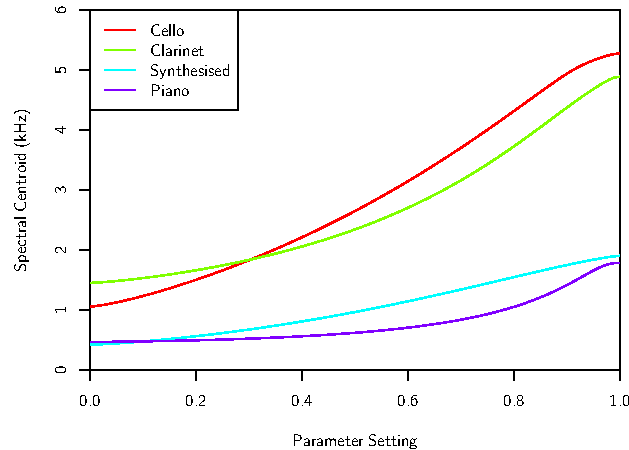
\includegraphics{chapter6/Images/MoveCentroids.pdf}
				\caption{Manipulating the spectral centroids of the test signals.}
				\label{fig:MoveCentroids}
			\end{figure}

			When $P$ is set to zero the input signal is effectively processed by only a low pass filter,
			reducing its spectral centroid. As $P$ is increased more energy is introduced in the higher
			harmonics until the maximum spectral centroid is reached at $P = 1$. For each signal the range of
			values the spectral centroid can take covers approximately two octaves. The spectral structure of
			the two bands determines how the spectral centroid changes within this range.

		\subsubsection*{Parameterisation of The Higher Order Spectral Moments}
			Higher order spectral moments are more difficult to parameterise as the measures depend on the
			displacement of each spectral component from the centroid. Skewness and kurtosis measurements also
			depend on the spectral spread. To simplify the control of these moments it is necessary to use
			manipulations which do not alter the moments they depend on. 
			
			Controlling the spread while keeping the centroid constant involves adding or removing energy
			symmetrically about the centroid. Deciding where to add or remove this energy is a non-trivial
			problem. The frequencies of the spectral components are not likely to be symmetrical about the
			centroid meaning different gains must be applied to components either side of the centroid.
			Calculating these gains must be done on a signal by signal basis making if difficult to provide a
			general solution. These problems are compounded further when trying to control the higher order
			moments as the spectral spread must also be kept constant.

			Intuition about what the spectral moments describe can be used to influence them in a simpler
			manner. These methods do not provide precise control over a specific moment but allow it to be
			increased or decreased.  Furthermore, they will have an effect on all the spectral moments rather
			than one in isolation. 
			
			Spectral spread can be increased by adding energy at frequencies which are more that one spectral
			standard deviation from the spectral centroid or reducing the energy at frequencies within one
			standard deviation of the centroid. Applying the opposite operations will decrease the spectral
			spread. This can be implemented using a system similar to that in
			Figure~\ref{fig:TwoBandSpectralCentroidSystem}. A band of harmonic energy is generated by
			processing the isolated $f_{0}$ with a nonlinear device followed by a band pass filter. This new
			band can then be summed with the original signal at the desired gain. Figure~\ref{fig:MoveSpreads}
			shows the change in spectral spread when the gain, $m$, of a spectral band, containing energy
			between $0.8\mu_{s}$ and $1.2\mu_{s}$, is changed.

			\begin{figure}[h!]
				\centering
				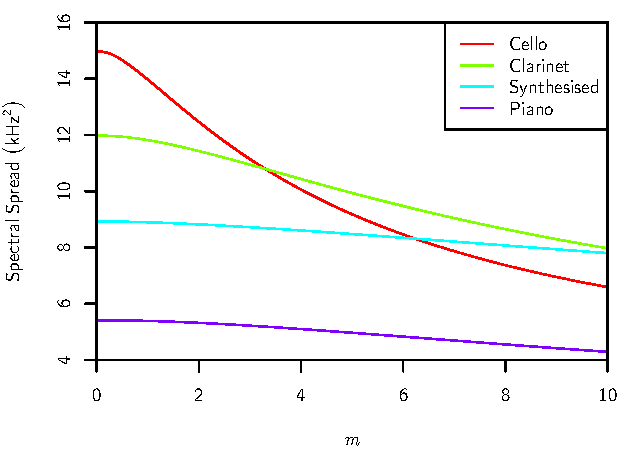
\includegraphics{chapter6/Images/MoveSpreads.pdf}
				\caption{Manipulating the spectral spreads of the test signals.}
				\label{fig:MoveSpreads}
			\end{figure}

			This is a manipulation in which an excitation system has an advantage over linear filtering. The
			ability to generate new bands of energy means that energy can be added near to the spectral
			centroid regardless of whether there was energy there in the input signal.

			Spectral skewness can be increased by applying a spectral tilt about the spectral centroid. A tilt
			with a positive gradient will decrease the skewness, whereas a negative gradient will increase the
			skewness. While the simplest system to achieve this would be a linear filter, an excitation based
			approach can provide a more flexible system in terms of manipulation or preservation of other
			features. Using the system shown in Figure~\ref{fig:SuperpositionSystem} a spectral tilt of $k$ dB
			per octave can be applied to the first nine harmonics. This is done by multiplying each harmonic's
			amplitude by $10^{\frac{k}{20}\log_{2} \left( \frac{\nu_{n}}{\mu_{s}} \right)}$. Increasing the
			value of $k$ increases the gradient of the tilt applied and thereby lowers the signal's spectral
			skewness. Figure~\ref{fig:MoveSkewnesses} shows the effects of changing $k$ when processing the
			test signals.

			\begin{figure}[h!]
				\centering
				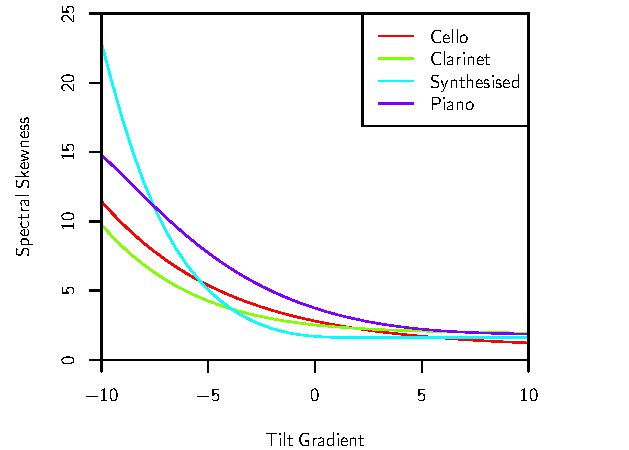
\includegraphics{chapter6/Images/MoveSkewnesses.pdf}
				\caption{Manipulating the spectral skewnesses of the test signals.}
				\label{fig:MoveSkewnesses}
			\end{figure}

			Only controlling the amplitudes of the first nine harmonics imposes restrictions on how the
			spectral skewness can be manipulated. The great amount of control over the low end of the signal's
			spectrum allows for skewness to be easily increased, as evidenced by
			Figure~\ref{fig:MoveSkewnesses}.  Decreasing the skewness however, is more difficult. The
			excitation system does not provide such fine control over the high end of a signal's spectrum.
			Using the spectral tilt method with a high positive value for $k$ will greatly attenuate the low
			order harmonics but leave the high order harmonics unprocessed. This means the output skewness will
			be equal to the skewness of the high order harmonics of the signal. This is seen in
			Figure~\ref{fig:MoveSkewnesses} where the skewness values all approach some minimum value.
			Introducing more high frequency energy using a nonlinear device, as done when controlling the
			spectral centroid, is a possible solution to this.

			Spectral kurtosis can be changed using the same method as for spectral spread. Increasing the
			energy near the centroid reduces the kurtosis, while removing energy near the centroid increases
			the kurtosis. Figure~\ref{fig:MoveKurtoses} shows the effect on the spectral kurtosis of the test
			signal when undergoing the same processing as described for Figure~\ref{fig:MoveSpreads}.
			
			\begin{figure}[h!]
				\centering
				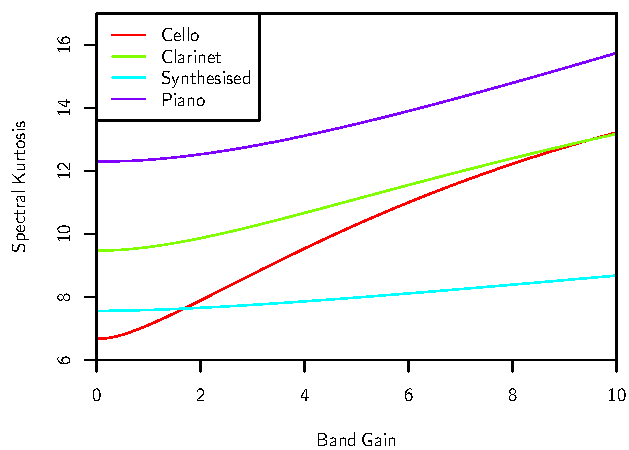
\includegraphics{chapter6/Images/MoveKurtoses.pdf}
				\caption{Manipulating the spectral kurtoses of the test signals.}
				\label{fig:MoveKurtoses}
			\end{figure}

	\subsection{Spectral Irregularity}
	\label{sec:FeatureControl-Parameterisation-Irregularity}
		\citet{beauchamp2007analysis} proposes methods for manipulating the spectral irregularity in additive
		synthesis systems. In effect these involve filtering of the frequency domain representation of a signal,
		applying a filter to the amplitudes of the signal's spectral components. This does not allow the
		irregularity to be set to a precise value but gives control over the direction in which the irregularity
		will change. Low pass filtering of the spectral components' amplitudes will decrease the irregularity while
		a high pass filter will do the opposite.
		
		Both the Krimphoff and Beauchamp irregularities (Equations \ref{eq:KrimphoffIrregularity} and
		\ref{eq:BeauchampIrregularity}) are based on the differences between each partial's amplitude and the mean
		amplitude of itself and the two partials surrounding it. Intuitively this value can be increased or reduced
		by moving the amplitudes of the partials away or towards their mean. To implement this using the system
		shown in Figure~\ref{fig:SuperpositionSystem} the new amplitudes of the first nine harmonics can be
		calculated using Equation~\ref{eq:PartialSmoothing}

		\begin{equation}
			a'_{n} = a_{n} \left( \frac{\sum_{k = 1}^{9} a_{k}}{9a_{n}} \right) ^{P}
			\label{eq:PartialSmoothing}
		\end{equation}

		Where $a'_{n}$ is the new amplitude of the $n$\super{th} partial, $a_{n}$ is the amplitude of the
		$n$\super{th} partial in the input signal, and $P$ is a parameter controlling how the irregularity is
		affected. Negative values of $P$ will increase the irregularity, while small positive values of $P$ will
		decrease the irregularity. The minimum possible irregularity is achieved when $P \approx 1$, higher values
		of $P$ will increase the irregularity again. Figure~\ref{fig:MoveIrregularities} shows how each of the
		spectral irregularity measures are affected by changes in the value of $P$.

		\begin{figure}[h!]
			\centering
			\captionsetup[subfigure]{oneside,margin={1cm, 0cm}}
			\subfloat[Krimphoff Irregularity]
			{
				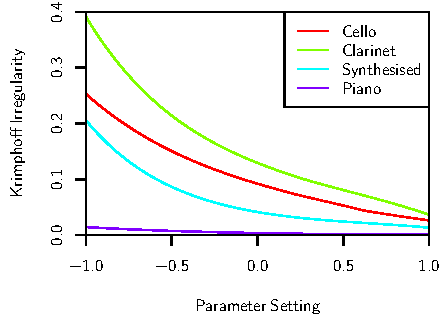
\includegraphics{chapter6/Images/MoveIrregularitiesK.pdf}
				\label{fig:MoveIrregularitiesK}
			}
			\quad
			\subfloat[Jensen Irregularity]
			{
				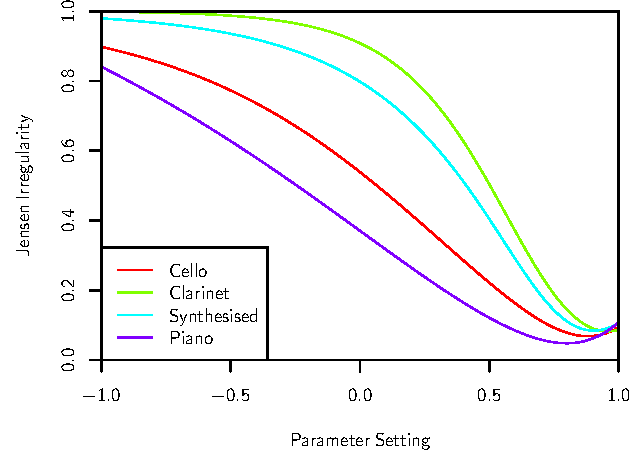
\includegraphics{chapter6/Images/MoveIrregularitiesJ.pdf}
				\label{fig:MoveIrregularitiesJ}
			}
			
			\subfloat[Beauchamp Irregularity]
			{
				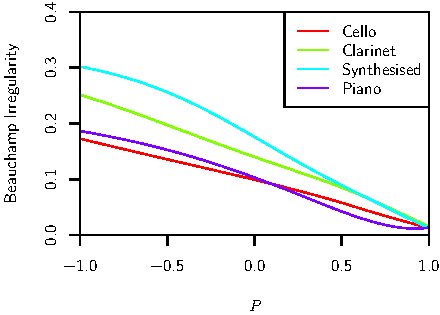
\includegraphics{chapter6/Images/MoveIrregularitiesB.pdf}
				\label{fig:MoveIrregularitiesB}
			}
			\caption{Manipulating the spectral irregularities of the test signals.}
			\label{fig:MoveIrregularities}
		\end{figure}

		As is most notable in Figure~\ref{fig:MoveIrregularitiesJ} the value of $P$ which will give the minimum
		flatness depends on the input signal. This is because only the first nine harmonics of each signal are
		being manipulated. The existing irregularity in the higher order harmonics may mean that adjusting the
		first nine harmonics to have the same level, as happens when $P = 1$, will not produce the minimum
		irregularity. The unbounded nature of the Krimphoff irregularity is also visible in
		Figure~\ref{fig:MoveIrregularities}.  While the Jensen and Beauchamp irregularities both asymptotically
		approach a maximum as $P$ is reduced the Krimphoff irregularity increases exponentially.

		Achieving this using excitation requires an analysis / resynthesis approach, replacing the existing
		spectral components with excited ones and changing the amplitudes to give the desired irregularity. If the
		analysis stage is removed the complexity of the system can be greatly reduced. The amplitudes of the newly
		excited spectral components can be predetermined and the irregularity manipulated as per
		Equation~\ref{eq:PartialSmoothing}. A different number of spectral components can be replaced with excited
		ones depending on how large a timbral variation is desired. Replacing only a few spectral components will
		provide a small amount of control over irregularity while preserving most of the spectrum of the input
		signal. Replacing more spectral components provides more control over the overall irregularity at the cost
		of losing more spectral information from the original.

		An alternate way to influence the irregularity of a signal is through control of the oddness and evenness
		as discussed in Section~\ref{sec:FeatureControl-Parameterisation-HarmonicParityRatio}. A signal with a high
		oddness and low evenness (or vice versa) will have a high a spectral irregularity whereas a signal with a
		more even distribution of energy between odd and even harmonics will have a lower irregularity. This allows
		the irregularity of a signal which contains both parities of harmonics can be changed by altering the
		signals oddness or evenness.

	\subsection{Spectral Flatness}
	\label{sec:FeatureControl-Parameterisation-Flatness}
		Spectral flatness is related to spectral irregularity. Many of the techniques to reduce the irregularity
		will also increase the flatness. More precisely, any manipulation which moves the amplitudes of all
		spectral components closer to each other will increase the spectral flatness. To take an example from
		Section~\ref{sec:FeatureControl-Parameterisation-Irregularity}, using a low pass filter on the amplitudes
		of the spectral components will increase the flatness of the spectrum.

		As the measure of spectral flatness (Equation~\ref{eq:Flatness}) is the ratio of the geometric and
		arithmetic means of the power spectrum, a greater degree of control can be achieved over it by altering one
		of the means while the other remains constant. The method discussed here changes the arithmetic mean while
		preserving the geometric mean. Consider two disjoint sets, $L$ and $H$, which are each composed of the
		indices of $k$ spectral components of the signal, such that the total energy in the spectral components
		denoted by $L$ is less than that of the spectral components denoted by $H$. A gain $m$ is applied to the
		spectral components denoted by set $H$ and the reciprocal gain $\frac{1}{m}$ applied to the spectral
		components denoted by set $L$. The resulting spectral flatness is calculated using
		Equation~\ref{eq:FlatnessManipulation}.

		\begin{gather}
			P = \left\{ n | n \in \textbf{N} \land n \leq N \right\} \nonumber \\
			E = P \setminus (L \medcup H) \nonumber \\
			A_{L} = \sum_{n \in L} a_{n}^{2} \quad A_{H} = \sum_{n \in H} a_{n}^{2}
			   \quad A_{E} = \sum_{n \in E} a_{n}^{2} \nonumber \\
			\mathrm{SF} = \frac{N\sqrt[N]{\prod_{n \in P} a_{n}^{2}}}
					   {\frac{A_{L}}{m^{2}} + m^{2}A_{H} + A_{E}}
			\label{eq:FlatnessManipulation}
		\end{gather}

		The spectral flatness can be increased by using a value of $m$ such that $\sqrt{\frac{A_{L}}{A_{H}}} < m <
		1$. The maximum possible flatness which can be achieved with the selected spectral components occurs when
		$m = \sqrt[4]{\frac{A_{L}}{A_{H}}}$. To decrease the spectral flatness a value of $m$ satisfying $0 < m <
		\sqrt{\frac{A_{L}}{A_{H}}}$ or $m > 1$ should be used. When $m = \sqrt{\frac{A_{L}}{A_{H}}}$ the arithmetic
		mean is unchanged, this provides a point at which the energy has been redistributed in the spectrum but the
		spectral flatness remains the same. 

		The gain value, $m$, can be calculated from a simplified control parameter, $P$, using
		Equation~\ref{eq:FlatnessControlParameter}. When $P$ is equal to 0 or 1 the spectral flatness will be
		unchanged.  Values of $P$ between 0 and 1 will increase the spectral flatness, with the maximum flatness
		being achieved at $P = 0.5$. Finally, when $P > 1$ the spectral flatness will decrease.
		Figure~\ref{fig:MoveFlatnesses} shows the effects of altering this parameter on the spectral flatness of
		the test signals when both sets, $L$ and $H$, are comprised of the indices of three spectral partials.

		\begin{equation}
			m = \sqrt{ \left( \frac{A_L}{A_H} \right) ^{1 - P}}
			\label{eq:FlatnessControlParameter}
		\end{equation}

		\begin{figure}[h!]
			\centering
			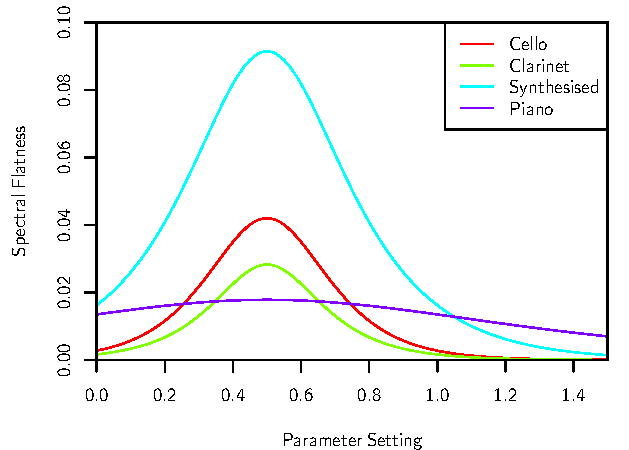
\includegraphics{chapter6/Images/MoveFlatnesses.pdf}
			\caption{Manipulating the spectral flatnesses of the test signals.}
			\label{fig:MoveFlatnesses}
		\end{figure}

		The maximum flatness which can be achieved depends on the flatnesses of the two sets $L$ and $H$.  If these
		sets are themselves flat (i.e. all partials in them have similar amplitudes) the maximum possible flatness
		will be large. If the amplitudes of partials within each set have high variance the capacity for increasing
		the overall flatness is reduced.

		Equation~\ref{eq:FlatnessManipulation} provides control over the spectral flatness in a signal where the
		amplitudes of the spectral components are known. As with control of spectral irregularity, an analysis /
		resynthesis technique could be utilised to implement this using harmonic excitation.  Again it is desirable
		to remove the analysis step in order to reduce the complexity of the system.  This can be done by replacing
		a band of spectral components with excited ones. Once a band has been replaced with excited components, the
		levels of these components can then be manipulated to change the flatness of the entire signal. Altering
		the flatness of the excited band using the method in Equation~\ref{eq:FlatnessManipulation} allows the
		overall flatness of the output to be influenced. Reducing the arithmetic mean of the power spectrum of the
		excited band also reduces the arithmetic mean of the power spectrum of the output signal. Thus, increasing
		the flatness of the excited band will also increase the flatness of the output signal and decreasing the
		flatness of the band decreases the flatness of the output signal.

		As the spectral flatness measure doesn't depend on the frequencies of the spectral components, deciding
		what two groups of components to apply reciprocal gains to will depend on the desired effect on other
		spectral features. For instance, to have a maximal effect on the odd to even harmonic ratio one could
		select two groups which consist of odd and even harmonics respectively. To have a minimal effect on this
		feature the two groups can both consist of one parity of harmonic.

	\subsection{Spectral Slope}
	\label{sec:FeatureControl-Parameterisation-Slope}
		As discussed in Section~\ref{sec:ExcitationEvaluation-Comparison-SpectralCharacteristics}, the spectral
		slope of the band of distortion components generated using a static nonlinearity depends on the continuity
		of the nonlinearity's characteristic curve and its derivatives. Using a simple system, similar to that
		shown in Figure~\ref{fig:F0Tracking}, the characteristic curve of the nonlinearity can be changed to
		influence the spectral slope of the output signal. While this would be very efficient, the spectral roll
		off of the output of a static nonlinearity can only be changed in increments of approximately 6dB per
		octave, reducing the precision of the control. The introduction of a static nonlinearity will also involve
		the generation of orders of harmonics which may not be desired.

		The system shown in Figure~\ref{fig:SuperpositionSystem} provides more control, allowing for slopes other
		than multiples of 6dB per octave. As with the discussions on spectral irregularity and flatness, an
		analysis / resynthesis approach provides finer control. To increase the spectral slope by $k$dB per Hz,
		each spectral component in the signal should have its amplitude, $a_{n}$, multiplied by the value
		$10^{\frac{k}{20}(\nu_{n} - \nu_{1})}$. If measuring spectral slope in dB per octave, increasing the slope
		by $k$dB per octave can be achieved by multiplying the amplitude of each spectral component in the signal
		by $10^{\frac{k}{20}\log_{2} \left( \frac{\nu_{n}}{\nu_{1}} \right)}$. As the excitation system can only
		individually control the individual amplitudes of the first nine harmonics, the gain for the high band
		(generated by the nonlinear device) is calculated using the frequency of the tenth harmonic.
		Figure~\ref{fig:MoveSlopes} shows the manipulation of the spectral slopes of the test signals by applying a
		tilt of $k$dB per octave.

		\begin{figure}[h!]
			\centering
			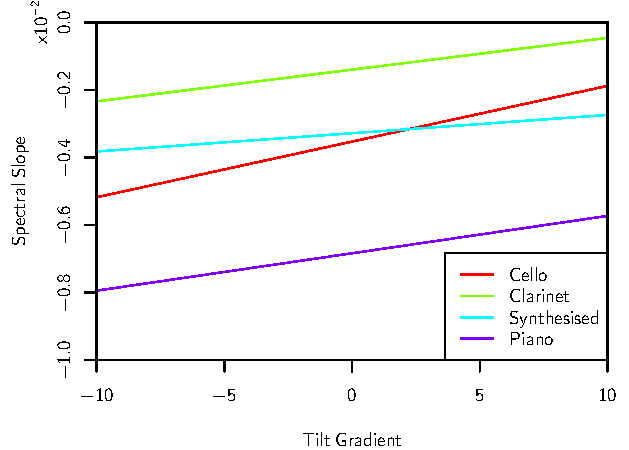
\includegraphics{chapter6/Images/MoveSlopes.pdf}
			\caption{Manipulating the spectral slopes of the test signals.}
			\label{fig:MoveSlopes}
		\end{figure}

		Ideally, each line in Figure~\ref{fig:MoveSlopes} would have the same gradient, as the signals' spectral
		slopes are being increased by the same amount. They do not however, as only the fist nine harmonics are
		being individually manipulated. The differences in amplitudes of the higher order harmonics between the
		signals accounts for the differences in control of the spectral slope.

		The complexity of the system can once again be reduced by removing the analysis stage of the processing.
		The amplitudes of the original harmonics and spectral slope of the high band can be set to produced the
		desired output slope. As with the control of other features, this decrease in complexity is achieved at the
		cost of losing spectral information from the original signal such as the orders of harmonics.

	\subsection{Tristimulus}
	\label{sec:FeatureControl-Parameterisation-Tristimulus}
		A generalised form of the tristimulus metrics measures the amplitude ratio, $R$, of a specific set of
		spectral components, $S$, and a set which includes that set, $F$. This is shown in
		Equation~\ref{eq:GeneralTristimulus}.

		\begin{gather}
			A = \sum_{n \in F} a_{n} \nonumber \\
			B = \sum_{n \in S} a_{n}, \quad S \subseteq F \nonumber \\
			R = \frac{B}{A}
			\label{eq:GeneralTristimulus}
		\end{gather}

		This ratio can be adjusted by applying gain to the spectral components in $S$. To attain a particular value
		of $R$ the required gain, $m$, can be calculated using Equation~\ref{eq:GeneralTristimulusManipulation}.

		\begin{equation}
			m = \frac{R(B - A)}{B(R - 1)}, \quad 0 \leq R < 1
			\label{eq:GeneralTristimulusManipulation}
		\end{equation}

		Similar to the method discussed for controlling spectral centroid, control of tristimulus metrics involves
		altering the energy in specific bands. A reduced version of the system shown in
		Figure~\ref{fig:SuperpositionSystem} can be used to control this. The system need only have individual
		control over the levels of the first four harmonics so the exciters for the fifth through ninth harmonics
		can be removed.

		The first tristimulus measure is easily controlled through applying gain to the isolated $f_{0}$.  The
		other two measures can be controlled in different ways depending on the requirements of the system.
		Individually controlling the levels of the second through fourth harmonics allows the second tristimulus
		measure to be manipulated while a more general nonlinear device can be used to generate higher order
		harmonics, changing the third tristimulus. As with the spectral centroid, using excitation to achieve this
		provides more flexibility as the tristimulus can be changed while preserving other features. For example,
		if the odd to even harmonic ratio needs to remain the same, but the second tristimulus change, different
		amounts of excitation can be applied to the second through fourth harmonics.

		Figure~\ref{fig:MoveTristimulus1} shows how the first tristimuli of the test signals changes when the gain,
		$m$, is applied at their isolated $f_{0}$ using the system shown in Figure~\ref{fig:SuperpositionSystem}.

		\begin{figure}[h!]
			\centering
			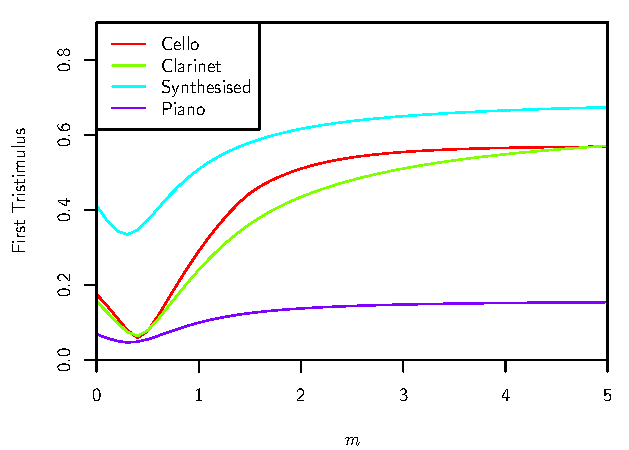
\includegraphics{chapter6/Images/MoveTristimulus1.pdf}
			\caption{Manipulating the first tristimuli of the test signals.}
			\label{fig:MoveTristimulus1}
		\end{figure}

		The maximum achievable first tristimulus value is determined by both the content of the input signal and
		the order of the filters used in the implementation of the excitation system. The system used for the
		values shown in Figure~\ref{fig:MoveTristimulus1} used second order IIR filters. This means that the
		isolated $f_{0}$ signal contains energy in some of the higher order spectral partials. In sounds where the
		$f_{0}$ has significantly less amplitude than subsequent spectral partials this is particularly
		problematic. The piano signal used for testing illustrates this. In this case the isolated $f_{0}$ signal
		has more energy in the second harmonic than at the $f_{0}$, severely reducing the maximum value which the
		first tristimulus can attain. Using higher order filters will alleviate this problem at the cost of
		increased processing complexity. The order of the filters is also responsible for the initial decrease in
		tristimulus value for small values of $m$. The $f_{0}$ is removed from the original signal using a high
		pass filter. The lower order this filter is, the more of a remnant of the $f_{0}$ remains. This initial
		decrease in the first tristimulus is due to destructive superposition between the isolated $f_{0}$ and this
		remnant.  Again, increasing the order of the filters used in the system will reduce these effects.

		\begin{figure}[h!]
			\centering
			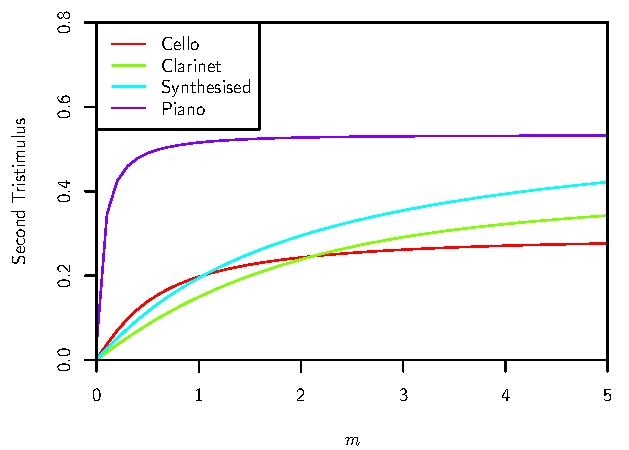
\includegraphics{chapter6/Images/MoveTristimulus2.pdf}
			\caption{Manipulating the second tristimuli of the test signals.}
			\label{fig:MoveTristimulus2}
		\end{figure}

		Control of the second tristimulus can be achieved with the same system, this time applying a gain, $m$, to
		the second, third and fourth excited harmonics. Figure~\ref{fig:MoveTristimulus2} shows how the second
		tristimulus value changes with $m$. As with control of the first tristimulus, the order of the filters used
		determines the maximum value the second tristimulus will take. The relationship is a more complex one
		however, as there is a nonlinear element to the system. The isolated $f_{0}$ signal will contain some
		energy at higher order partials.  When this signal is used to generate new harmonics some of the
		intermodulation components will be higher in frequency than the desired harmonic. This results in more
		energy being introduced above the fourth harmonic, reducing the maximum possible second tristimulus.

		The third tristimulus is more easily controlled using the same system as used for controlling the spectral
		centroid (Figure~\ref{fig:TwoBandSpectralCentroidSystem}). A band of high order harmonics is generated from
		the isolated $f_{0}$ using a static nonlinearity and a high pass filter.  Figure~\ref{fig:MoveTristimulus3}
		shows how changing the gain, $m$, of this band effects the third tristimulus of the test signals.

		\begin{figure}[h!]
			\centering
			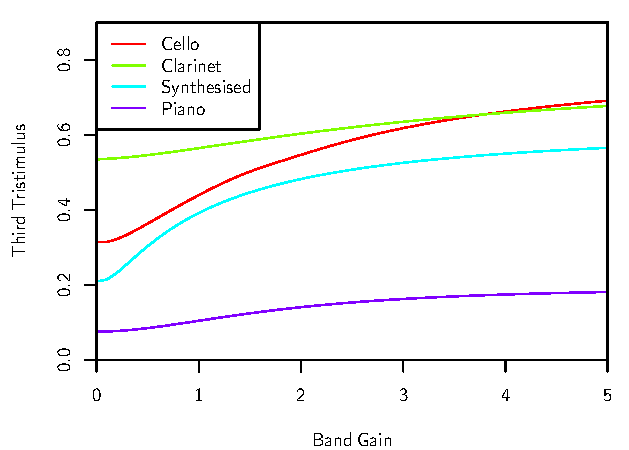
\includegraphics{chapter6/Images/MoveTristimulus3.pdf}
			\caption{Manipulating the third tristimuli of the test signals.}
			\label{fig:MoveTristimulus3}
		\end{figure}

		Again, second order IIR filters have been used to filter out the lower order harmonics from the excited
		signal.	These low order filters do not remove all the energy in the first 4 harmonics thereby limiting how
		high the third tristimulus can be made.

	\subsection{Odd to Even Harmonic Ratio}
	\label{sec:FeatureControl-Parameterisation-HarmonicParityRatio}
		The odd to even harmonic ratio, Equation~\ref{eq:HarmonicParityRatio}, can easily be altered by applying
		gain to only the odd harmonics. To change the ratio to a particular value, $\mathrm{OER}$, the required
		gain, $m$, is calculated using Equation~\ref{eq:HarmonicParityRatioManipulation}.

		\begin{equation}
			m = \sqrt{\frac{\mathrm{OER}\sum_{1 \leq n \leq N, n \text{ is even}} h_{n}^{2}}
				       {\sum_{1 \leq n \leq N, n \text{ is odd}} h_{n}^{2}}},
				       \quad \mathrm{OER} \geq 0
		       \label{eq:HarmonicParityRatioManipulation}
		\end{equation}

		If instead, separate control of the oddness and evenness of a signal is desired, Equations \ref{eq:Oddness}
		and \ref{eq:Evenness}, can be generalised to give Equation~\ref{eq:GeneralOddness}.

		\begin{gather}
			A = \sum_{n \in F} a_{n}^{2} \nonumber \\
			B = \sum_{n \in S} a_{n}^{2}, \quad S \subseteq F \nonumber \\
			R = \sqrt{\frac{B}{A}}
			\label{eq:GeneralOddness}
		\end{gather}

		Like Equation~\ref{eq:GeneralTristimulus} this measures the ratio of amplitudes of a set of frequencies and
		a larger set of frequencies which contains that set. This time using the squares of the amplitudes and
		taking the square root afterwards. The value of the ratio can be altered by applying gain to the spectral
		components in the set $S$. The required gain factor, $m$, to give a ration of $R$ is calculated using
		Equation~\ref{eq:GeneralOddnessManipulation}.

		\begin{equation}
			m = \sqrt{\frac{R^{2}(B - A)}{B(R^{2} - 1)}}, \quad 0 \leq R < 1
			\label{eq:GeneralOddnessManipulation}
		\end{equation}

		For control over the oddness or evenness of a signal, a system which provides control over individual
		harmonics is not necessary. While this level of control allows for more complex manipulations a simpler
		system can be employed in which separate bands of odd and even order harmonics are generated. Such a system
		is shown in Figure~\ref{fig:HarmonicParitySystem}. This system uses two parallel static nonlinearities to
		generate two signals consisting of only odd harmonics and even harmonics respectively. The properties of
		these nonlinearities can be adjusted to shape the spectra of each of these signals which are further shaped
		through linear filtering. The gains of these two signals allow control over the oddness and evenness of
		the signal using Equation~\ref{eq:GeneralOddnessManipulation}.

		\begin{figure}[h!]
			\centering
			\begin{tikzpicture}
				\node (In) at (-1, -2.25) {$x[n]$};
				\coordinate (InMid) at (0, -2.25);
				\draw (In) -- (InMid);

				\coordinate (Side) at (0, -1.25);
				\draw (InMid) -- (Side);

				\node (F0) [draw] at (2, -1.25) {$f_{0}$ Tracker};
				\node (F0Filter) [draw] at (2, -2.25) {BPF};
				\draw (InMid) -- (F0Filter);
				\draw (F0) -- (F0Filter);
				\draw (Side) -- (F0);

				\node (Add) [operator] at (11.5, -2.25) {+};

				\coordinate (ExciterIn) at (4, -2.25);
				\draw (F0Filter) -- (ExciterIn);

				% odd harmonics
				\coordinate (OddIn) at (4, -1.25);
				\node (Odd) [draw] at (6, -1.25) {Odd Harmonics};
				\draw (OddIn) -- (Odd);

				\node (OddFilter) [draw] at (8.5, -1.25) {Filter};
				\draw (Odd) -- (OddFilter);

				\node (OddGain) [gain] at (10, -1.25) {};
				\draw (OddFilter) -- (OddGain);
				\coordinate (OddOut) at (10.5, -1.25);
				\draw (OddGain) -- (OddOut);
				\draw (OddOut) -- (Add);

				% even harmonics
				\coordinate (EvenIn) at (4, -2.25);
				\draw (OddIn) -- (EvenIn);
				\node (Even) [draw] at (6, -2.25) {Even Harmonics};
				\draw (EvenIn) -- (Even);

				\node (EvenFilter) [draw] at (8.5, -2.25) {Filter};
				\draw (Even) -- (EvenFilter);

				\node (EvenGain) [gain] at (10, -2.25) {};
				\draw (EvenFilter) -- (EvenGain);
				\coordinate (EvenOut) at (10.5, -2.25);
				\draw (EvenGain) -- (EvenOut);
				\draw (EvenOut) -- (Add);

				% through
				\coordinate (Through) at (0, -3.25);
				\draw (InMid) -- (Through);
				\node (ThroughFilter) [draw] at (8.5, -3.25) {Filter};
				\draw (Through) -- (ThroughFilter);
				\node (ThroughGain) [gain] at (10, -3.25) {};
				\draw (ThroughFilter) -- (ThroughGain);
				\coordinate (ThroughOut) at (10.5, -3.25);
				\draw (ThroughGain) -- (ThroughOut);
				\draw (ThroughOut) -- (Add);

				\node (Out) at (12.75, -2.25) {$y[n]$};
				\draw (Add) -- (Out);
			\end{tikzpicture}
			\caption{A system to control the levels of odd and even order harmonics individually.}
			\label{fig:HarmonicParitySystem}
		\end{figure}

		The odd and even harmonics in a signal could be separated using linear filters. This approach requires in
		depth analysis of the signal adding complexity and possible delay to the system but has some advantage in
		preservation of signal characteristics. When using excitation this complexity is reduced but the problems
		discussed in Section~\ref{sec:FeatureControl-Systems-Superposition} become apparent. To elicit full control
		over the levels of the odd and even harmonics using the system shown in
		Figure~\ref{fig:HarmonicParitySystem} all the harmonic content in the output signal is generated by the
		nonlinearities. This is likely to cause a dramatic change in timbre as most of the information present in
		the original signal has been replaced. 

		A method to counteract this is to only excite even or odd harmonics in the signal at any one time.  The
		relative levels of odd and even harmonics can still be adjusted but some more of the original signal's
		spectral shape is preserved. Avoiding superposition still remains difficult in this situation as it would
		mean filtering out alternate harmonics in the input signal. Allowing superposition to occur sacrifices
		precise control in order to maintain some of the input's characteristics.

		An example of how the system in Figure~\ref{fig:HarmonicParitySystem} can be used is as follows.  The
		isolated $f_{0}$ of each test signal is processed by two parallel static nonlinearities. A band of odd
		order harmonics is generated through a hard peak clipper and a band of even order harmonics through full
		wave rectification of this clipped signal. The band of even order harmonics is high pass filtered in order
		to remove the energy introduced at 0Hz by rectification. Both bands of harmonics are then low passed
		filtered with a cutoff at the frequency of the ninth harmonic and the original signal is high pass filtered
		at the same frequency. The ninth harmonic is chosen due to it being the highest individually resolved
		harmonic as discussed in Section~\ref{sec:FeatureControl-Systems-SpectralShaping}. The three signals are
		then summed at different ratios to control the evenness or oddness of the output.
		Figure~\ref{fig:MoveParities} shows the effects of manipulating the levels of odd and even order harmonics
		in this way. The original signal remains at unity gain whereas the gains of the harmonic bands are
		determined by a parameter, $P$.  Odd order harmonics are multiplied by a gain of $P$ and even order
		harmonics by $1 - P$.

		\begin{figure}[h!]
			\centering
			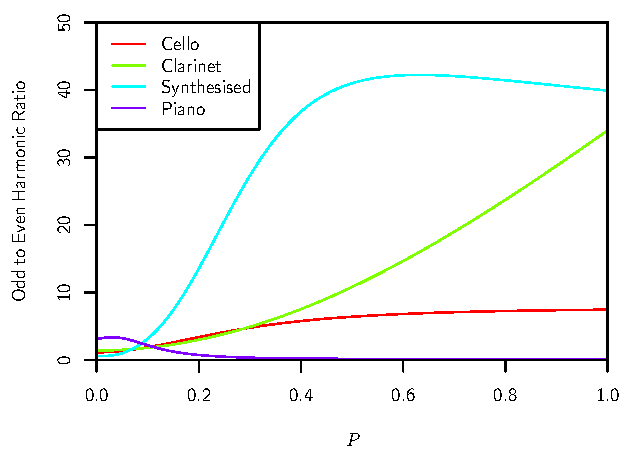
\includegraphics{chapter6/Images/MoveParities.pdf}
			\caption{Manipulating the odd to even harmonic ratios of the test signals.}
			\label{fig:MoveParities}
		\end{figure}

		Here we see how the spectral content of the input signal influences the effects of the processing.  The
		$\mathrm{OER}$ of the clarinet signal seems to be the easiest to control. This can be attributed to the
		high oddness of the unprocessed clarinet signal, the $f_{0}$ is easier to isolate because there is very
		little energy in the second harmonic. With a better isolated $f_{0}$ the two bands of excited harmonics
		will be better separated with respect to the parities of harmonics they contain.

		The cello and synthesised signals both exhibit a limit on how high the $\mathrm{OER}$ can be made. This
		is due to both bands of excited harmonics containing both parities of harmonic.  The general upward trend
		for both signals illustrates that the two bands generated do contain the majority of their energy in the
		correct parity harmonics but higher order filtering of the $f_{0}$ is needed to better segregate them. The
		decrease in $\mathrm{OER}$ seen for the synthesised signal is due to destructive superposition between
		the harmonics in the three signals being summed.

		The system discussed here provides no control over the $\mathrm{OER}$ of the piano signal. This is again
		due to the low amplitude $f_{0}$. The isolated $f_{0}$ signal contains the majority of its energy in the
		second harmonic. This causes the two bands of generated harmonics to both contain mostly even order
		harmonics, meaning the resulting signal will have a high evenness, or low $\mathrm{OER}$.

	\subsection{Inharmonicity}
	\label{sec:FeatureControl-Parameterisation-Inharmonicity}
		While it is reasonably simple to introduce inharmonicity in harmonic excitation systems, controlling the
		inharmonicity of a signal is a more complicated problem. The system shown in
		Figure~\ref{fig:InharmonicitySystem} can be use to apply multiple approaches to this problem. 

		A simple two band approach leaves the lower partials of the system unaltered and generates a high band
		using a static nonlinearity and filtering. The inharmonicities in this high band will be amplified versions
		of those in the original signal. This approach is not applicable in a number of situations, such as when
		the input only contains perfectly harmonic partials or when the desired result is is to reduce the
		inharmonicity in a signal.
		
		The opposite system, in which the high frequencies are left unaltered and the low frequency partials are
		generated individually, provides a greater amount of control over the inharmonicity of the resulting
		signal. The newly generated partials can be given frequencies closer to harmonics than those in the input
		signal reducing the overall inharmonicity. It also allows for generation of inharmonic partials in a signal
		with zero inharmonicity. This system is more complicated both in computation and use. Because the
		inharmonicity metric (Equation~\ref{eq:Inharmonicity}) depends on the frequencies of every partial, there
		are numerous ways a signal can be manipulated resulting in the same value for the inharmonicity. When
		manipulating the inharmonicity a decision needs to be made as to which partials are to be made inharmonic
		and by how much. One method of deciding this is to model it on the vibrational modes of an acoustic
		instrument, ensuring a natural set of inharmonic partials. To increase the inharmonicity, the frequencies
		of the partials can be moved from being harmonic towards the frequencies indicated by the model. One such
		model is that given by \citet{rossing2002the} for calculating the frequencies of the spectral partials of
		piano strings. In this model the frequencies of each partial are determined by an inharmonicity factor,
		$A$, using Equation~\ref{eq:PianoInharmonicity}. In the modelling of piano timbre the value of $A$ is
		calculated from the physical properties of the piano string. For creative purposes the value of $A$ can be
		arbitrarily set.

		\begin{equation}
			a_{n} = nf_{0} \left( 1 + \left( n^{2} - 1 \right) A \right)
			\label{eq:PianoInharmonicity}
		\end{equation}

		Using the system shown in Figure~\ref{fig:InharmonicitySystem} the inharmonicities of the first nine
		harmonics of a signal can be set according to this model. Figure~\ref{fig:MoveInharmonicities} shows how
		the resulting inharmonicity changes with the inharmonicity factor $A$.

		\begin{figure}[h!]
			\centering
			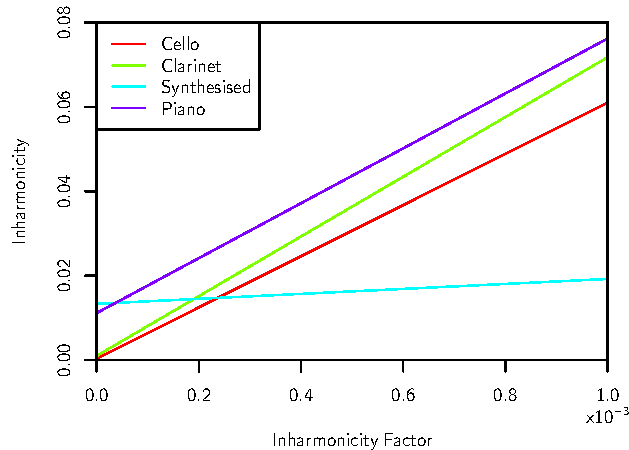
\includegraphics{chapter6/Images/MoveInharmonicities.pdf}
			\caption{Manipulating the inharmonicities of the test signals.}
			\label{fig:MoveInharmonicities}
		\end{figure}

		As only the first nine harmonics are being altered, the degree to which the inharmonicity can be
		manipulated depends on the spectral content of the input signal. The partials of the synthesised signal
		have amplitudes which roll off at a very low rate, meaning there is significant energy in the partials
		above the ninth order. The frequencies of these partials will then have a more significant impact on the
		inharmonicity of the signal. Because the frequencies of these partials is not being altered this reduces
		the range of values which the resulting inharmonicity can take. The other three signals all have higher
		spectral roll off, such that the influence of their existing high order partials has a smaller effect on
		the overall inharmonicity. The issue of higher order harmonics reducing the maximum inharmonicity could be
		counteracted by adding an addition frequency shifter to the system. This shifter would operate on the
		filtered input signal and shift all the higher order partials by the same amount.

\section{Conclusions}
\label{sec:FeatureControl-Conclusions}
	This section has presented and discussed how harmonic excitation can be used to control specific audio features in
	harmonically structured signals. Methods have been suggested by which a single parameter can be mapped to the
	parameters of the harmonic excitation systems proposed in Section~\ref{sec:FeatureControl-Systems} to control the
	value of a particular audio feature in the output. Where possible the parameter has been defined such that with a
	little analysis of the input signal, the value of the feature in the output can be precisely set. In other cases
	the parameter is defined such that the function describing the relationship between the parameter and feature
	values is monotonic. In the case of spectral flatness this was not possible, but the parameter values at which the
	maximum spectral flatness occurs is defined. The function describing spectral flatness as the parameter is moved
	away from this value is monotonically decreasing. While these parameterisations do not allow for the absolute value
	of an audio feature to be defined, the user is given control over the direction in which the feature is altered.
	This allows them to be used for timbral transformations in which the semantic descriptor is defined by a particular
	change in feature values, such as for `bright' and `warm' (Chapter~\ref{chap:TimbreEvaluation}).

	In implementing these methods further challenges are met. The parameterisations all rely on the $f_{0}$ of the
	input signal being perfectly isolated and the elimination of superposition for any of the excited harmonics
	(Section~\ref{sec:FeatureControl-Systems-Superposition}). In real time systems this will not always be possible.
	The implementations used when processing the test signals used second order IIR filters for these tasks to
	investigate the effects this would have when processing different signals. As seen in the figures in
	Section~\ref{sec:FeatureControl-Parameterisation} this less than ideal filter performance produces non-monotonic
	behaviour for some of the systems. This is especially notable when controlling the odd to even harmonic ratio of
	the piano signal, due to the nature of the damped fundamental the system was only able to produce even order
	harmonics when using a low order filter. In most of these cases increasing the order of the filters will improve
	the control over the audio feature at the expense of increasing computational complexity.

	Other nonlinearities and deviations from monotonic behaviour in the parameterisations can be accounted for by the
	fact that only the first nine harmonics are being controlled individually. While this is based on psychoacoustic
	principles, as discussed in Section~\ref{sec:FeatureControl-Systems-SpectralShaping}, the audio features
	manipulated are not. Equal magnitude changes in an audio feature due to spectral changes at different frequencies
	will not have the same perceived effect. Individual control of the first nine harmonics gives control over the most
	perceptually relevant portion of the spectrum. Inaccuracies in the control of features due to lack of control over
	higher order harmonics are deemed to be less important than those due to filtering of signals to isolate the
	$f_{0}$ and avoid superposition.

	In the following chapter perceptual listening tests are undertaken to asses how well the methods proposed in this
	chapter can be used to provide perceptually control of audio. Firstly the best method are exciting individual
	harmonics is determined. Then the systems discussed here are specialised to apply the same feature manipulations as
	those described by a particular descriptor in the SAFE dataset (Chapter~\ref{chap:TimbreEvaluation}).
